\documentclass{report}

\usepackage{subcaption} % package for subfigures
\usepackage{hyperref}  % package for linking figures etc
\usepackage{enumitem}  % package for description with bullets
\usepackage{graphicx}  % package for importing images
\usepackage{mathtools} % package for math equation
\usepackage{mathrsfs}  % package for math font
\usepackage{indentfirst} % package for getting ident after section or paragraph
\usepackage[export]{adjustbox}
% \usepackage{amsmath}

\setlength{\parindent}{2em} % how much indent to use when we start a paragraph

\graphicspath{ {./theory/figures/} }       % path for images

\begin{document}

\chapter{Introduction}
Nowadays, the enormous increase of computing power help us deal with a lot of difficult situations appeared in our daily life.
A lot of areas of science have managed to tackle with problems, which were consided non trivial 20 years ago. One of
these area is Computer Vision and an import problem is human action recognition and localization.
\section{Problem statement}
The area of human action recognition and locatization has 2 main goals:
\begin{enumerate}
\item Automatically detect and classify any human activity, which appears in a video.
\item Automatically locate in the video, where the previous action is performed.
\end{enumerate}

\subsection{Human Action Recognition}
Considering human action recognition, a video may be consisted of only by 1 person doing something, however, this is a ideal
situation. In most cases, videos contain multiple people, who perform multiple actions or may not act at all in some segments.
So, our goal is not only to classify an action, but to dertemine the temporal boundaries of each action.
\subsection{Human Action Localization}
Alongside with Human Action Recognition, another problem is to present spatial boundaries of each action. Usually, this means
presenting a 2D bounding box for each video frame, which contains the actor. Of course, this bounding box moves alongside with
the actor.

\section{Applications}
The field of Human Action Recognition and Localization has a lot of applications which include 
 content based video analysis,automated video segmentation, security and surveillance systems,
human-computer interaction.

The huge availability of data (especially of videos) create the  necessity to find ways to take advantage of them.
About 2.5 billion images are uploaded in Facebook every month, more than 34K hours of video in YouTube and
about 5K images every minutes. On top of that, there are about 30 million surveillance cameras in US, which means
about 700K video hours per day. All those data need to be seperated in categories according to their content in
order to search them more easily. This process takes places by hand, by the user who attaches
keywords or tags, however, most users avoid to do so. This situation creates the need to create algorithms for
automated indexing based on the content of the video.

Another application is video summury. This area take place usually in movies or sports events. In movies,
video analysis algorithms can create a small video containing all the important moments of the movie. This
can be achieve by choosing video segments which an important action take place such as killing the villain
of the movie. In sports events, video summury applications include creating highlight video automatically.

On top of that, human action recognition can replace human operators in surveillance systems. Until now,
security systems include a system of multiple cameras handled by a human operator, who judges if a person
is acting normally or not. Automatic action classification systems can act like human, and immediately
judge if there is any human behavioral anomaly.

Last but not least, another field of application is related with human-computer interaction. Robotic applications
help elderly people deal with their daily needs. Also, gaming applications using Kinect create new kinds of
gaming experience without the need of a physical game controller.

\section{Challenges and Datasets}
The wide variety of applications creates a lot of challenges which involve with action recognition systems.
The most important include large variations in appearence of the actors, camera view-point changes, occlusions
non-rigid camera motions etc. On top of that, a big problem is that there are too many action classes which means
that manual collection of training sample is prohibitive. Also, some times, action vocabulary is not well defined.
As figure \ref{fig:open_example} shows, ``Open'' action can include a lot of kinds of actions, so we must carefully
choose which granularity of the action we will consider.

\begin{figure}[h]
  \centering
  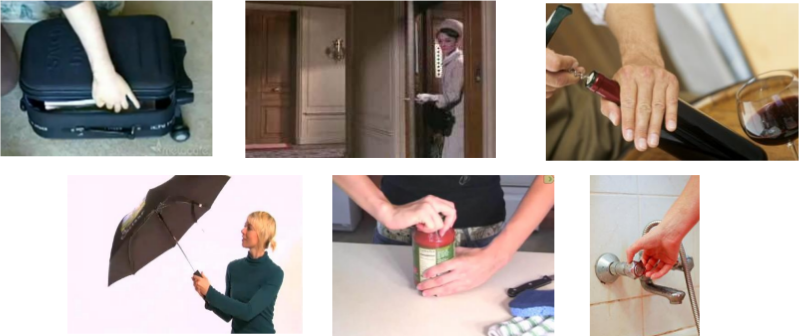
\includegraphics[scale=0.3]{open_example}
  \caption{Examples of ``Open'' action}
  \label{fig:open_example}

\end{figure}

In order to deal with those challenges, several standard action datasets have been created in order to delevop
robust human action recognition systems and detection algorithms.
The first datasets like KTH\cite{} include 1 actor performing using a static camera over homogeneous backgrounds.
Even though, those datasets help us design the first action recognition algorithms, they were not able to deal with the above
challenges.
This lead us to design datasets containing more ambigious videos such as Joint-annotated Human Motion Database(JHMDB)\cite{}
and UCF-101\cite{}.
\subsection{JHMDB Dataset}
The JHMDB dataset (\cite{Jhuang:ICCV:2013}) is a fully annotated dataset for human actions and human poses. It is consisted of 21 action categories and 928
clips extracted from Human Motion Database (HMDB51) \cite{Kuehne11}. This dataset contains trimmed videos with duration between
15 to 40 frames. Each clip is annotated for each frame using a 2D pose and contains only 1 action.
In order to train our model for action localization, we modify 2D poses into 2D boxes containing the whole pose in each frame.
There are available 3 different splits for training data, proposed by the authors. We chose the first split which contains 660
videos for training set and 268 for validation . 

\subsection{UCF-101 Dataset}
The UCF-101 dataset(\cite{soomro2012ucf101} contains 13320 videos from 101 action categories.
From those, for 24 classes and 3194 video spatio-temporal annotations are included. This means for each frames in which an action is taking place,
there is a 2D bounding box surrounding the actor.  We seperate them in 2284 videos for training set and 910 for validation test according to the
first proposed training split. For training data, there are videos up to 641 frame while in validation data max number of frames is 900.
Each video,both training and validation, is, of course, untrimmed,  including more than 1 simultaneous actions. We took annotations from
\cite{singh2016online} because the proposed, by the authors, annotations contains some mistakes.

\section{Motivation ans Contibutions}
The current achievements in Object Recognition Networks and in 3D Convolution Networks for Action Recognition have triggered us to try
to combine them in order to achieve state-of-the-art results for action localization. We introduce a new network structure inspired by
\cite{DBLP:journals/corr/HouCS17}, \cite{DBLP:journals/corr/abs-1712-09184},\cite{Ren:2015:FRT:2969239.2969250} and for implementation
by \cite{jjfaster2rcnn}.

Our contributions are the following 1) We create a new framework for action localization extending the code taken from faster RCNN,
2) We try to create a network for proposing sequences of bounding boxes in video clips which may containg an anction taking advantage
of the spatio-temporal features which 3D Convolutions provide us, 3) We create a connection algorithm for linking these sequences of
bounding boxes in order to propose a final action tube and 4) we try to find the most suitable feature maps for classifying them.

\section{Thesis structure}
The rest of Thesis is organized as follows. Chapter 2 provides an general introduction to Machine Learning techniques currently used.
Chapter 3 presents an overview of literature on human action recognition and localization. Chapter 4 introduces the first basic
element of our system, Tube Proposal Network (TPN) and shows all the approachs designed for this system. Chapter 5 proposes an algorithm
for linking the proposed TOIs from every video segment. In Chapter 6, we can see the results for classification and detection of our system,
using 2 classic clasifiers. Chapter 7 is used for conclusions, summury of our contribution alongside with possible future work.


\end{document}
